\section{Orbits in an axisymmetric potential}
Considering an axisymmetric potential for a simple model of a galaxian disk first proposed by Toomre (1964, ApJ):
\begin{equation}
    U(r) = -(1+r^2)^{-1/2},
\end{equation}

the equation of motion is given by
\begin{equation}
    F=-\frac{dU(r)}{dr}=-\frac{r}{(1+r^2)^{3/2}}.
\end{equation}

This is a differential equation that can be solved using leapfrog integration.

\begin{figure*}[h!]
    \centering
    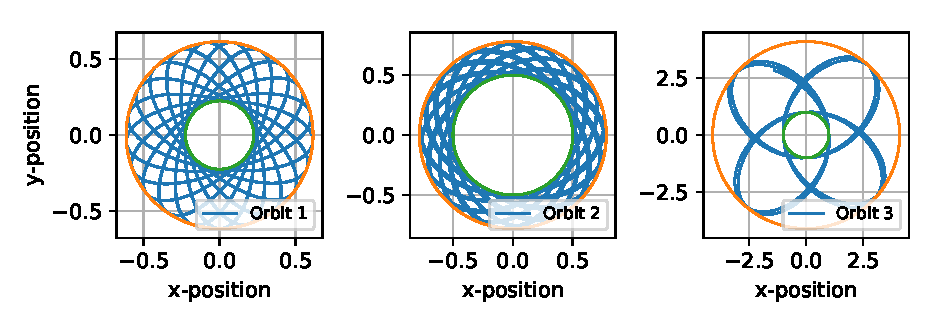
\includegraphics{CodeAndFigures/ToomrePotentialOrbits.pdf}
    \caption{Rosette Orbits using initial conditions of Left: $x=.3$, $y=0$, $v_x=.3$ and $v_y=.4$ Middle: $x=0$, $y=0.5$, $v_x=.6$ and $v_y=0$. Right:$x=1$, $y=0$, $v_x=0$ and $v_y=1$.}
    \label{fig:ToomreOrbits}
\end{figure*}

Using the initial values listed on table \ref{tab:ToomreOrbits}, we can calculate the orbits for each case. Figure \ref{fig:ToomreOrbits} shows that the orbits are not close but they precess. These types of orbits are called rosette orbits because of the shape or tube orbits because they have an inner and outer boundary.

\begin{table}[]
    \centering
\begin{tabular}{lrrrrrr}
\toprule
{} &    x &    y &  $v_x$ &  $v_y$ &  $r_{inner}$ &  $r_{outer}$ \\
\midrule
Orbit 1 & 0.30 & 0.00 &   0.30 &   0.40 &         0.22 &         0.61 \\
Orbit 2 & 0.00 & 0.50 &   0.60 &   0.00 &         0.50 &         0.78 \\
Orbit 3 & 1.00 & 0.00 &   0.00 &   1.00 &         1.00 &         4.10 \\
\bottomrule
\end{tabular}

    \caption{Caption}
    \label{tab:ToomreOrbitIV}
\end{table}

These systems have two conserved quantities, the total energy $E_T$ and angular momentum $L$. Using the initial conditions, one can calculate the total energy of the system,
\begin{equation}
    E_T=K + U(r) = \frac{1}{2}v^2 + U(r)
\end{equation}
where U is the potential energy and K is the kinetic energy of the initial values, and the angular momentum by
\begin{equation}
    L=r^2\Dot{\theta}
\end{equation}
where 
\begin{align}
    r^2 = x^2 + y^2\\
    \Dot{\theta} = r \times \dot{r}\\
    \dot{r}^2 = v_x^2 + v_y^2
\end{align}.

Figure \ref{fig:conservedQuants} shows the total energy and the angular momentum of these rosette orbits are being conserved through time. 
\begin{figure*}[h]
    \centering
    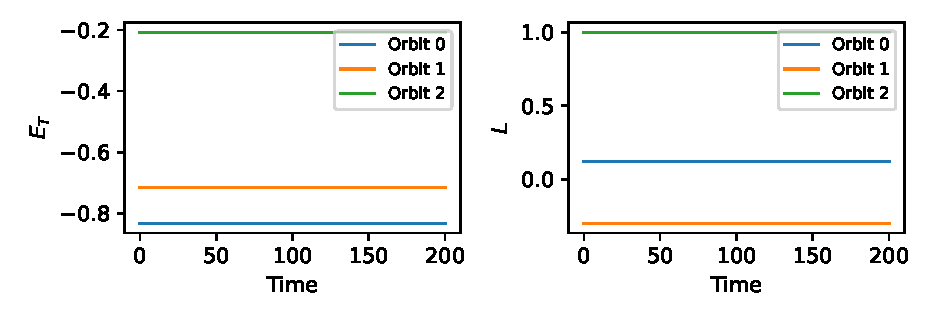
\includegraphics{CodeAndFigures/EnergyMomentumPlot.pdf}
    \caption{Left: Energy and Right: Angular Momentum of the rosette orbits in function with time.}
    \label{fig:conservedQuants}
\end{figure*}

The inner and outer radius of the orbits are found by finding the roots of
\begin{equation}
    E_T - U(r) - \frac{L^2}{r^2} = 0
    \label{eq:rootfunc}
\end{equation}

The bisect method was used to find the roots. The bisect methods finds the roots of a given function within a range of values to evaluate the function. The range for $r$ was determined by first plotting the equation \ref{eq:rootfunc} and determining visually were a sign change occurred. The value for inner and outer radius for each trial orbit is listed in table \ref{tab:ToomreOrbits} and is shown in Figure \ref{fig:ToomreOrbits} in orange and green. 




